\documentclass[11pt,a4paper]{ivoa}
\input tthdefs

\usepackage{listings}
\lstloadlanguages{sh,make,[latex]tex}
\lstset{flexiblecolumns=true,numberstyle=\small,showstringspaces=False,
  identifierstyle=\texttt,defaultdialect=[latex]tex,language=tex}

\usepackage{todonotes}
\usepackage{float}
\usepackage{adjustbox}
\usepackage{lscape}

\usepackage[english]{babel}

\usepackage[utf8]{inputenc}

\usepackage{booktabs,xcolor}
\definecolor{texcolor}{rgb}{0.4,0.1,0.1}
\definecolor{lightgray}{gray}{0.9}

\lstloadlanguages{SQL}
\lstset{flexiblecolumns=true,basicstyle=\ttfamily}

\iftth
  \newcommand{\BibTeX}{BibTeX}
\fi

\hyphenation{Obs-Core}

\title{Observation Locator Table Access Protocol}

\ivoagroup{Data Model Working Group}

\author{Aitor Ibarra}
\author{Jesús Salgado}
\author{Matthias Ehle}
\author{Carlos Gabriel}
\author{James Dempsey}
\author{Markus Demleitner}
\author{María Díaz Trigo}
\author{Karl Foster}
\author{Jaime Kennea}
\author{Mark Kettenis}
\author{Peter Kretschmar}
\author{Erik Kuulkers}
\author{Giorgio Matt}
\author{Bruno Merín}
\author{Marco Molinaro}
\author{Jan-Uwe Ness}
\author{Julian Osborne}
\author{Emma de Oña Wilhelmi}
\author{Edward J. Salbol}
\author{Emilio Salazar}
\author{Celia Sánchez}
\author{Richard Saxton}
\author{Gregory Sivakoff}
\author{Lian Tao}
\author{Mark Taylor}
\author{Aaron Tohuvavohu}
\author{Bill Workman}

\editor{Jesús Salgado}
\editor{Aitor Ibarra}



\begin{document}

\begin{abstract}

  The Observation Locator Table Access Protocol (ObsLocTAP)
  defines a data model for scheduled observations and a method to run
  queries over compliant data, using several Virtual Observatory
  technologies.

  The data model builds on the ObsCore data model, removing elements
  associated with dataset access that are not available during the planning phase.
  In this way, this standard is focused on access to metadata related
  to the planning of a certain observatory, more than on access to the
  scientific data products. Also, the data model will be focused on discovery
  of planned observations, which is very useful information for
  multi-wavelength coordination observations, re-planning information
  propagation, follow-up of Targets of Opportunity alerts, preparation of
  proposals, etc.

  As with ObsCore, a serialisation into a relational table is defined, which
  allows users to run complex queries using the IVOA Table Access Protocol.
  The document also prescribes how to register and discover ObsLocTAP services.

\end{abstract}

\section*{Acknowledgments}
The authors acknowledge the comments from Observatories members and from the
IVOA members in general.


\section*{Conformance-related definitions}

The words ``MUST'', ``SHALL'', ``SHOULD'', ``MAY'', ``RECOMMENDED'', and
``OPTIONAL'' (in upper or lower case) used in this document are to be
interpreted as described in IETF standard RFC2119 (\citealt{std:RFC2119}).

The \emph{Virtual Observatory (VO)} is a
general term for a collection of federated resources that can be used
to conduct astronomical research, education, and outreach.
The \href{http://www.ivoa.net}{International
Virtual Observatory Alliance (IVOA)} is a global
collaboration of separately funded projects to develop standards and
infrastructure that enable VO applications.

\section*{Role within the VO Architecture}

%%%%%%%%%%%%%%%%%%%% Figure/Image No: 1 starts here %%%%%%%%%%%%%%%%%%%%

\begin{figure}
\centering

% As of ivoatex 1.2, the architecture diagram is generated by ivoatex in
% SVG; copy ivoatex/archdiag-full.xml to archdiag.xml and throw out
% all lines not relevant to your standard.
% Notes don't generally need this.  If you don't copy archdiag.xml,
% you must remove archdiag.svg from FIGURES in the Makefile.

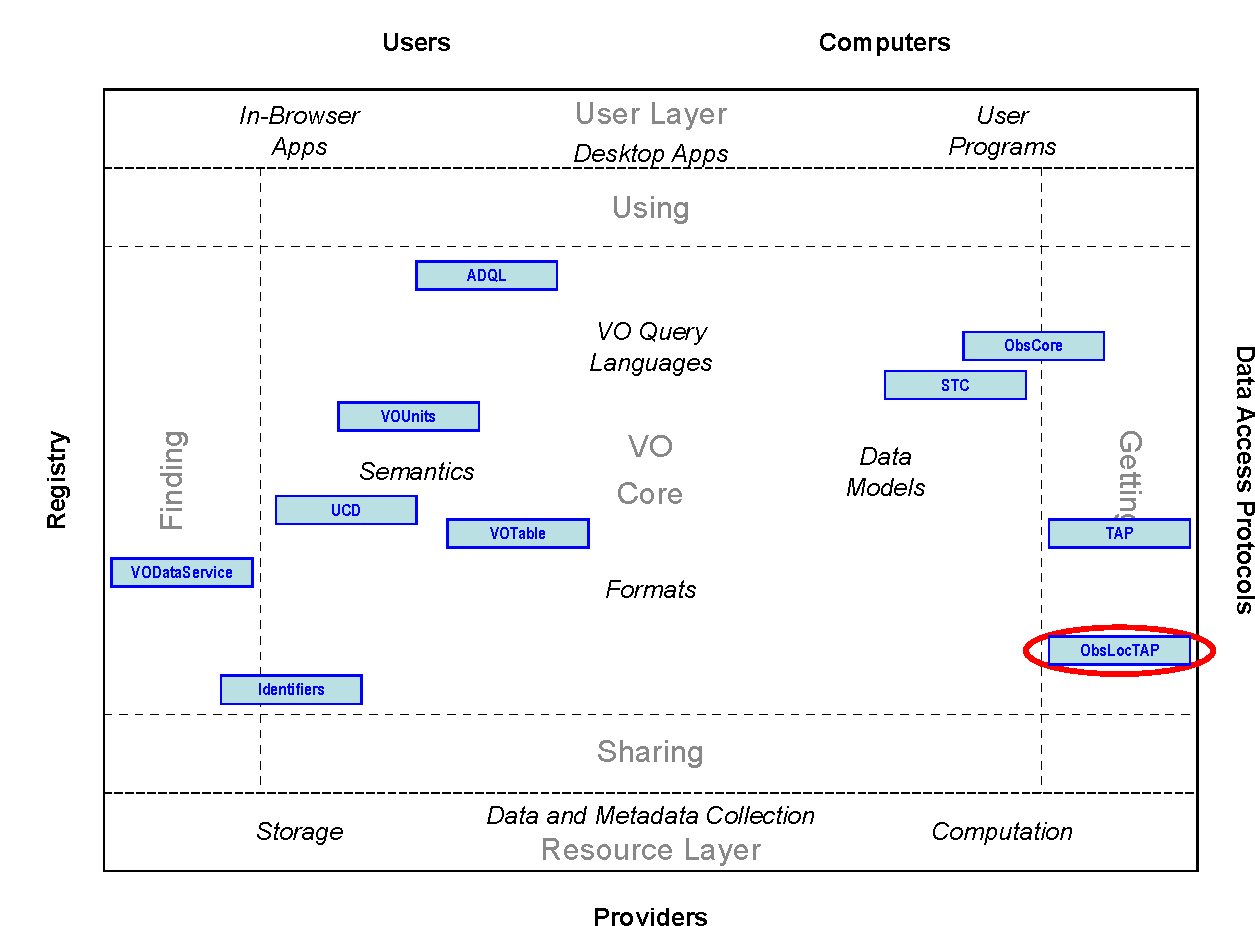
\includegraphics[width=0.9\textwidth]{role_diagram.pdf}
\caption{Architecture diagram for this document}
\label{fig:archdiag}
\end{figure}


%%%%%%%%%%%%%%%%%%%% Figure/Image No: 1 Ends here %%%%%%%%%%%%%%%%%%%%
Fig.~\ref{fig:archdiag} shows the role ObsLocTAP plays within the
IVOA architecture \citep{note:VOARCH}. ObsLocTAP reuses various model elements (including geometrical entities) of ObsCore and, 
as ObsCore itself, relies on the TAP specification to deploy its relational content.
Also, queries are written following ADQL as the query language and the default result is defined
in VOTable format, including units in a VOUnits compatible format, UCDs to
describe columns and Identifiers to point to the data model. Finally, ObsLocTAP
services can be registered making use of the VODataService standard format.

\pagebreak


\section{Overview}
The \textbf{Observation Locator Table Access Protocol} (ObsLocTAP henceforth)
specifies in a standard format, services to retrieve information about planned,
scheduled and performed observations of a given target (or coordinates) for a
given astronomical observatory based on the existing ObsCore data model. This
standard does not describe the access to data obtained after the processing of
the observational activity, as that is the goal of ObsCore (archived
observations), although the discovery could be done in a similar way.
Therefore, although there is some overlap on the data model described in both
standards, entities, use cases and communities are different.

In order to standardize the workflow of one observation, status is defined as
follows:
%%%%%%%%%%%%%%%%%%%% Figure/Image No: 0 starts here %%%%%%%%%%%%%%%%%%%%

\begin{figure}[H]
\advance\leftskip 0.0in		\hfill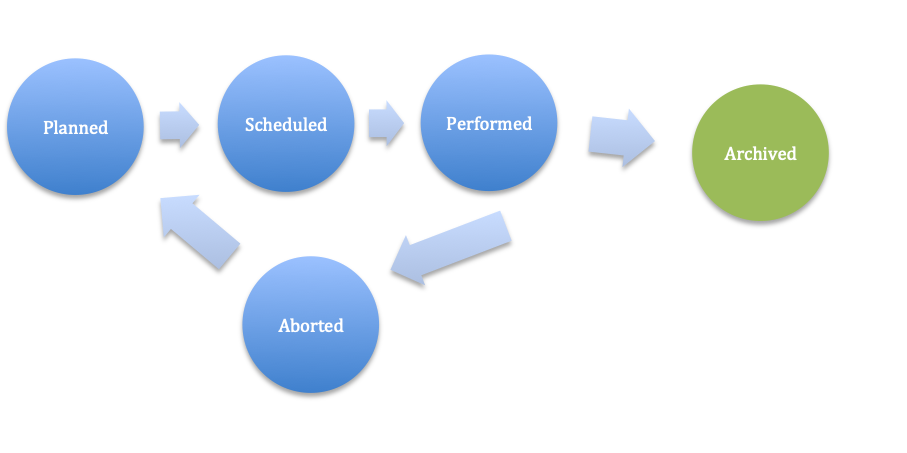
\includegraphics[width=5.0in]
{./media/observations_workflow.png}\hfill\strut%
\end{figure}
%%%%%%%%%%%%%%%%%%%% Figure/Image No: 1 starts here %%%%%%%%%%%%%%%%%%%%

\begin{itemize}
	\item{\textbf{Planned}: a possible observation, in most of the cases coming
  from a certain proposal, has been identified. There is not yet an association
  to a certain time period when the observation can be executed.}

	\item{\textbf{Scheduled}: mission planners allocate a certain period when the
	observation can be executed. Also, some changes could be expected on
  coordinates (due to some refinement) and other fields.}

	\item{\textbf{Unscheduled}: the observation has been removed from the schedule.   	     
	The observation could be recovered as planned into the planning log.}

	\item{\textbf{Performed}: the observation has been performed successfully.
  This is only at the operational level as there is not guarantee of scientific
  results.}

	\item{\textbf{Aborted}: the observation has not been correctly performed. 
	The observation could be recovered as planned into the planning log.}

	\item{\textbf{Archived}: the observation has data available and can be found
  in a science archive. This archived phase is the main target of the ObsCore
  specification, so it can be considered out of the scope of the present
  specification.}

\end{itemize}

This new standard would allow client applications to use a standardised VO
service to aggregate and display the information of former and future
observations. This new standard will help in the preparation of
multi-observatory multi-instrument observation campaigns, whose
coordination needs certain standards for efficient communication.

The ObsLocTAP interface makes use of the IVOA TAP (\citealt{2019ivoa.spec.0927D})
to access observational metadata. The IVOA TAP protocol is a powerful and quite
flexible system, easily adapted to a wide variety of use cases simply by
defining agreed-upon table structures. Users can write complex queries against these
using the common Astronomical Data Query Language (ADQL; \citealt{2008ivoa.spec.1030O})

There are several open source TAP implementations that could be used by the
community (minimizing the implementation effort for the observatories) and it
has been efficiently used in operational archives like, e.g., the Gaia Archive.

In the current document, we will focus on
the description of the Data Model, tables
and use cases. No deviation from standard TAP or ADQL is foreseen, where TAP
defines the mechanisms to exchange queries and data as well as error messages
and ADQL the query language syntax.

\section{Use cases}
The planning process can be usually described as follows (although observatories
can have different procedures to fulfill this process):

\begin{itemize}
	\item{The observatory receives observatory proposals from scientists that are
  reviewed by an expert panel (e.g., OTAC = Observing Time Allocation
  Committee).}

	\item{Proposals are ranked by their scientific relevance.}

	\item{Proposals are related to one or more observations that are inserted
  into the observation planning system of the observatory.}

	\item{Observation planners decide which observations can be scheduled in the
  short-medium plan trying to maximize the relevance of a certain observation
  period (e.g., per night or orbit revolution) and taking into account the
  constraints of the observatory (e.g., visibility of the object, geometrical
  constraints like the Sun or the Earth for space-based observatories, etc).}

	\item{In case of unexpected events like, e.g., targets of opportunity, the
  scheduled plan could be replaced by another one modifying the short or
  medium-term plans.}

\end{itemize}

Standardizing the way to publish this short/medium plan through ObsLocTAP
services provides higher scientific impact of the observing time, follow-up of
astronomical events and better cooperation between observatories. We present
here a selected list of use cases. Later in the document, we will show how
these use cases can be fulfilled using the current specification:

\subsection{Common tooling for observers across observatories}
Standardization of the publication of observing plans will facilitate the
implementation of a tool that lets observers monitor the progress of their
proposed observations that works for all observatories that adopt ObsLocTAP.
This kind of application has been requested by the community for a long time.
Ideally, that would obviate custom, per-observatory web forms, saving work for
observatories and observers alike.

\subsection{Avoiding unnecessary proposals for observation time}
An astronomer wants to propose an observation and can, before doing so,
globally determine if a possibly suitable observation is already scheduled.
This might prevent costly duplicate observations.

\subsection{Support for weighting proposals}
The bodies (e.g., OTAC) that decide on the observation schedule can use the
observation schedules of their own and other observatories to raise or lower
priorities on a given proposal. This might even take into account observation
histories, giving demerits to possibly unnecessary repeated observations.

\subsection{Identification of planned observations in a certain spectral range
for a certain astronomical event}
A scientist could be interested in the planned observations for a certain
astronomical object at different spectral ranges. For example, this is commonly
done in the GRB (Gamma Ray Burst) events follow-up, where the event is
decreasing in energy and multiple observations must be done in decreasing energy
order by different observatories to fully characterize the event.

By using ObsLocTAP services, users could discover and propose sequential
observations that will allow the future SED characterization of this
astronomical event.

\subsection{Follow-up of Targets of Opportunity}
Observing plans can be changed very fast due to targets of opportunity (ToOs).

There are two different types of ToOs in astronomy:
\begin{itemize}
	\item{Unpredictable ToOs: Astronomical events that require immediate or almost
  immediate observations and that may even require coordination between
  different observatories.}

	\item{Predictable ToOs: These astronomical events are related (not always) to
  known transient phenomena or due to coordinated observations of targets
  special interest.}

\end{itemize}

For the first type, the short-term plan can be affected in a very short time
scale, as when they trigger follow-up observations of a certain astronomical
event.

VOEvent initiatives are focused on the announcement of the astronomical event
and in the propagation of the information obtained due to follow-up
observations, but only when the observations are already executed. By the
implementation of ObsLocTAP services, the decision how short-term observing
plans are modified can be published live to the scientific community.

\subsection{Modification of the plans due to external conditions or anomalies}
Usually, observatory plans can be modified due to various reasons. They could be
changed by anomalies in the instruments, astronomical events, external
conditions, etc.
For ground-based observations, atmospheric conditions could imply
the modification of the planning, whereas for space-based observatories,
radiation due to solar flares could force observations to be stopped.

It is difficult for the scientist to follow-up the status of the plan. This
could be fulfilled by the implementation of ObsLocTAP services.

\section{Observation Locator Elements}
\subsection{Observation Locator data model }
In the IVOA ObsCore specification, two main data models are connected to
describe the data model behind most of the use cases needed to discover observed
datasets:

\begin{itemize}
	\item{Characterization: Provides a description of metadata associated to a
  certain observation. In particular, the different axes (e.g., the spatial
  axis, the time axis, spectral axis$ \ldots $ ) are used to describe the
  coverage of the observation on different observables.}

	\item{ObsDataSet: Provides support to discover data associated to a certain
  performed observation.}

\end{itemize}

In the case of planned (not executed) observations, only the Characterization
DM could be used, as the observations covered are not yet performed and hence
most of the metadata associated to the ObsDataSet will be empty. Also, the data
produced after the processing of the observational metadata could be not present
yet for recently executed observations and, in other cases, data could be
present only within the mission archive but not in the planning system.

Although it is correctly set in the ObsCore DM that the association multiplicity
between the Characterization DM and ObsDataSet is $0\ldots\ast$, the ObsCore
specification clearly considers that metadata related to the data access is set
for all the records. In the present document the data access metadata will not
be included.

Also, although some of the elements could be known a priori, it is difficult to
estimate the number of elements in the different axes (space, time, spectral,
\dots).
This implies that this information will not be present for most of the planning
lists. This is why this information has been removed as well from the present
data model.

That implies the data model for the use cases described in the present document
is reduced to:

%%%%%%%%%%%%%%%%%%%% Table No: 3 starts here %%%%%%%%%%%%%%%%%%%%
\begin{landscape}
\begin{table}
\def\hlstrut{\vrule height 13pt depth5pt width0pt}
\begin{tabular}{ |l|l|l|l| }
\hline
\hlstrut\textbf{Column Name} &
\hlstrut\textbf{Description} \\
\hline
%row no:2
t\_planning &
Time in MJD when this observation has been added or modified into the
planning log \\
\hline
%row no:3
target\_name &
Astronomical object observed, if any \\
\hline
%row no:4
obs\_id &
Observation ID \\
\hline
%row no:5
obs\_collection &
Name of the data collection \\
\hline
%row no:6
s\_ra &
Central right ascension, ICRS \\
\hline
%row no:7
s\_dec &
Central declination, ICRS \\
\hline
%row no:8
s\_fov  &
Diameter (bounds) of the covered region \\
\hline
%row no:9
s\_region &
Sky region covered by the data product (expressed in ICRS frame) \\
\hline
%row no:10
s\_resolution &
Spatial resolution of data as FWHM \\
\hline
%row no:11
t\_min &
Start time in MJD \\
\hline
%row no:12
t\_max &
Stop time in MJD \\
\hline
%row no:13
t\_exptime &
Total exposure time \\
\hline
%row no:14
t\_resolution &
Temporal resolution FWHM \\
\hline
%row no:15
em\_min &
Start in spectral coordinates \\
\hline
%row no:16
em\_max &
Stop in spectral coordinates \\
\hline
%row no:17
em\_res\_power &
Spectral resolving power \\
\hline
%row no:18
o\_ucd &
UCD of observable (e.g., phot.flux.density, phot.count, etc.) \\
\hline
%row no:19
pol\_states &
List of polarization states or NULL if not applicable \\
\hline
%row no:20
pol\_xel &
Number of polarization samples \\
\hline
%row no:21
facility\_name &
Name of the facility used for this observation \\
\hline
%row no:22
instrument\_name &
Name of the instrument used for this observation \\
\hline
%row no:23
obs\_release\_date &
Observation release date (ISO 8601) \\
\hline
%row no:24
t\_plan\_exptime &
Planned or scheduled exposure time \\
\hline
%row no:25
category &
Observation category. One of the following values: Fixed, Coordinated, Window, 
Other \\
\hline
%row no:26
priority &
Priority level $ \{ $ 0, 1, 2$ \} $ \\
\hline
%row no:27
execution\_status &
One of the following values:  Planned, Scheduled, Unscheduled, Performed, Aborted \\
\hline
\end{tabular}
\end{table}
\end{landscape}

%%%%%%%%%%%%%%%%%%%% Table No: 3 ends here %%%%%%%%%%%%%%%%%%%%
The obsplan table exposed by an ObsLocTAP service MUST include all 
the columns listed, even though null values may be permitted in some
of the columns. Additional non-standard columns are permitted in a 
particular obsplan table implementation.

The purpose of the observation locator query is to allow users/clients to
retrieve the information of planned observations of a particular target or
sky coordinates. The most basic query parameters will be the sky coordinates
(Right Ascension and Declination). Additional parameters may be used to
customize the visibility checks.

As can be seen, most of the data model elements come from the IVOA
Characterization data model and the exact description of these fields is
present in the IVOA ObsCore standard (\citealt{2017ivoa.spec.0509L}).

\textbf{\textit{s\_region}}, as described on IVOA ObsCore standard, can be
used to precisely specify the covered spatial region of a data product. The
s\_region geometrical field is allowed to be serialised according DALI 1.1
(\citealt{std:DALI}) specification or using a STC-S format
described on the section 6 of TAP 1.0 
(\citealt{2011ivoa.spec.1028T}). In
the WHERE clause, s\_region constraints will generally make use of ADQL
geometries (CIRCLE, POLYGON, POINT) and the geometry predicate functions
(CONTAINS, INTERSECTS).

In case the exact final region cannot be specified (e.g., because an undefined
position angle of the planned observation), s\_region can be approximated by
implementors as a CIRCLE with the center position as \textbf{s\_ra} and
\textbf{s\_dec} and a radius of \textbf{s\_fov}/2.

The planning time (\textbf{t\_planning}) has been added in order to allow the
discovery of the time when this observation (scientific entity) has been added
(or modified) to the plan, in order to let clients ask for changes in the plan
incrementally (i.e., without having to retrieve and compare locally the full set
of future observations with a previously download one).

The planning exposure time (\textbf{t\_plan\_exptime}) has been added in order
to show any possible inconsistency between the scheduled exposure time and the
real performed exposure time (\textbf{t\_exptime}). If an observation was
performed without problems, both quantities usually have the same values. Any
discrepancy between these two values could reflect problems or deviations between
scheduled observations and performed observations or a more accurate value.

The \textbf{category} element has been added in order to help users to identify
those observations that were scheduled in coordination with other facilities or
those observations that have to be executed at a fixed time.

The \textbf{priority} element has been added in order to help users to identify
those observations that were scheduled with a high priority (value=2) and
therefore cannot be removed from the planning or are hard to re-schedule. If the
observation can be easily shifted to a different time (value=0), the user could
query the service to identify this type of observations.

Execution status (\textbf{execution\_status}) provides a description of the current status of the planned
observation. Initially, observations are inserted as planned into the system.
The final state will be one of executed or aborted.

\subsection{Compulsory metadata}
In contrast to normal ObsTAP services where most of the metadata is compulsory,
in the case of ObsLocTAP, this cannot always be maintained. In some cases, the
target associated to the observations could still be confidential information
which needs to be hidden due to, e.g., observatory confidentiality constraints.

The same approach of hidden information status could also be applied to the
instruments or configurations used so the metadata should be present as follows:

\begin{itemize}
	\item{For confidential observations that need to be hidden from the planning
  point of view, the period should be shown as blocked. That means that an entry
  should appear with the start time, end time and duration as relevant. The
  facility name should also be provided.}

	\item{If the astronomical target is still hidden, coordinates and target
  should be set to \textit{null} in the obsplan table.}

	\item{Observational metadata about instrument, spectral coverage and
  polarization states should appear with a general default value, describing a
  non-detailed mode, but with values that are more general than the exact ones
  to be used during the real observation. For example, a general X-ray spectral
  coverage could appear in \textit{em\_min} and \textit{em\_max} for an X-ray
  observatory but not the exact details of the instrument mode that will be used
  for the confidential observation.}

	\item{Exact details of the observation could be updated whenever the
  observation passes from the hidden state to the public state from the
  metadata point of view.}

\end{itemize}

\subsection{Implementation of ObsLocTAP as a TAP service}
The primary access path to ObsLocTAP information is through TAP
(\citealt{2010ivoa.spec.0327D}) database queries. In order to fulfill some advanced
use cases, ObsLocTAP services MUST provide, at least, the following ADQL
(\citealt{2008ivoa.spec.1030O}) geometrical features: CIRCLE, POLYGON, INTERSECTS
and CONTAINS.\par

\subsection{TAP Schema}
The following table gives the entries for the ivoa.obsplan table in
TAP\_SCHEMA.columns

%%%%%%%%%%%%%%%%%%%% Table No: 4 starts here %%%%%%%%%%%%%%%%%%%%
\begin{landscape}
\begin{table}
\def\hlstrut{\vrule height 13pt depth5pt width0pt}
\begin{tabular}{ |l|l|l|l|l|l| }
\hline
%row no:1
\hlstrut\textbf{column\_name} &
\hlstrut\textbf{data type} &
\hlstrut\textbf{units} &
\hlstrut\textbf{utype} &
\hlstrut\textbf{UCD} \\
\hline
%row no:2
t\_planning &
(float) &
d &
&
\\
\hline
%row no:3
target\_name &
(string) &
&
Target.name &
meta.id;src \\
\hline
%row no:4
obs\_id &
(string) &
&
DataID.observationID &
meta.id \\
\hline
%row no:5
obs\_collection &
(string) &
&
DataID.collection &
meta.id \\
\hline
%row no:6
s\_ra &
(float) &
deg &
Char.SpatialAxis.Coverage.Location.Coord.Position2D.Value2.C1 &
pos.eq.ra \\
\hline
%row no:7
s\_dec &
(float) &
deg &
Char.SpatialAxis.Coverage.Location.Coord.Position2D.Value2.C2 &
pos.eq.dec \\
\hline
%row no:8
s\_fov &
(float) &
deg &
Char.SpatialAxis.Coverage.Bounds.Extent.diameter &
phys.angSize;instr.fov \\
\hline
%row no:9
s\_region &
(region) &
&
Char.SpatialAxis.Coverage.Support.Area &
pos.outline;obs.field \\
\hline
%row no:10
s\_resolution &
(float) &
arcsec &
Char.SpatialAxis.Resolution.Refval.value &
pos.angResolution \\
\hline
%row no:11
t\_min &
(float) &
d &
Char.TimeAxis.Coverage.Bounds.Limits.StartTime &
time.start;obs.exposure \\
\hline
%row no:12
t\_max &
(float) &
d &
Char.TimeAxis.Coverage.Bounds.Limits.StopTime &
time.end;obs.exposure \\
\hline
%row no:13
t\_exptime &
(float) &
s &
Char.TimeAxis.Coverage.Support.Extent &
time.duration;obs.exposure \\
\hline
%row no:14
t\_resolution &
(float) &
s &
Char.TimeAxis.Resolution.Refval.value &
time.resolution \\
\hline
%row no:15
em\_min &
(float) &
m &
Char.SpectralAxis.Coverage.Bounds.Limits.LoLimit &
em.wl;stat.min \\
\hline
%row no:16
em\_max &
(float) &
m &
Char.SpectralAxis.Coverage.Bounds.Limits.HiLimit &
em.wl;stat.max \\
\hline
%row no:17
em\_res\_power &
(float) &
&
Char.SpectralAxis.Resolution.ResolPower.refVal &
spect.resolution \\
\hline
%row no:18
o\_ucd &
(string) &
&
Char.ObservableAxis.ucd &
meta.ucd \\
\hline
%row no:19
pol\_states &
(string) &
&
Char.PolarizationAxis.stateList &
meta.code;phys.polarization \\
\hline
%row no:20
pol\_xel &
(integer) &
&
Char.PolarizationAxis.numBins &
meta.number \\
\hline
%row no:21
facility\_name &
(string) &
&
 Provenance.ObsConfig.Facility.name &
meta.id;instr.tel \\
\hline
%row no:22
instrument\_name &
(string) &
&
Provenance.ObsConfig.Instrument.name &
meta.id;instr \\
\hline
%row no:23
obs\_release\_date &
(date) &
&
Curation.releaseDate &
time.release;obs.exposure \\
\hline
%
%row no:24
t\_plan\_exptime &
(float) &
s &
Char.TimeAxis.Coverage.Support.Extent &
time.duration;obs.exposure \\
\hline
%row no:25
category &
(string) &
&
&
\\
\hline
%row no:26
priority &
(integer) &
&
&
\\
\hline
%row no:27
execution\_status &
(string)&
&
&
\\
\hline
\end{tabular}
\end{table}
\end{landscape}

%%%%%%%%%%%%%%%%%%%% Table No: 4 ends here %%%%%%%%%%%%%%%%%%%%
The concrete types used in the database and in table output are
up to the implementation, but the data type annotations above
must result in VOTable column output with {\tt datatype},
{\tt xtype} and {\tt arraysize} attributes as follows:
{\it (float)\/} means floating point values (numeric datatype);
{\it (integer)\/} means integer values (integer datatype);
{\it (string)\/} means string values (character datatype and a suitable arraysize);
{\it (date)\/} means Timestamp string values as described in DALI,
and
{\it (region)\/} means {\em either\/} an STC-S-format string
as described in section 6 of TAP 1.0,
{\em or\/} one of the region encodings such as Circle or Polygon
described in DALI.

\vspace{\baselineskip}
\section{Use Cases as TAP/ADQL queries}
In this section, we present ways to implement the use cases mentioned in the
first part of this note as ADQL queries to an ObsLocTAP service.

\subsection{Discovery of observations scheduled or planned for a certain
observatory}
Planned observations on a certain time period can be discovered using the
following ADQL query:

%%%%%%%%%%%%%%%%%%%% Table No: 5 starts here %%%%%%%%%%%%%%%%%%%%
\begin{lstlisting}[language=SQL]
SELECT * 
FROM ivoa.obsplan 
WHERE
  t_min < <end_time>
  AND t_max > <start_time>
\end{lstlisting}
%%%%%%%%%%%%%%%%%%%% Table No: 5 ends here %%%%%%%%%%%%%%%%%%%%
Where \textit{<start\_time>} and \textit{<end\_time> }are the minimum and
maximum times of the period to be requested in MJD. This query provides
observations that overlap with a certain time range, e.g.,

%%%%%%%%%%%%%%%%%%%% Table No: 6 starts here %%%%%%%%%%%%%%%%%%%%
\begin{lstlisting}[language=SQL]
SELECT *
FROM ivoa.obsplan
WHERE
  t_min < 58700
  AND t_max  > 58500
\end{lstlisting}
%%%%%%%%%%%%%%%%%%%% Table No: 6 ends here %%%%%%%%%%%%%%%%%%%%

To find observations planned between 2019-01-17 and 2019-08-05.

\subsection{Identification of planned observations in a certain spectral range
for a certain astronomical object}
Sending the same ADQL query to all the available ObsLocTAP servers can discover
planned observations that cover a certain spectral range:

%%%%%%%%%%%%%%%%%%%% Table No: 7 starts here %%%%%%%%%%%%%%%%%%%%
\begin{lstlisting}[language=SQL]
SELECT *
FROM ivoa.obsplan
WHERE
  t_min < <end_time>
  AND t_max > <start_time>
  AND em_min < <spectral_coordinate_max>
  AND em_max > <spectral_coordinate_min>
\end{lstlisting}
%%%%%%%%%%%%%%%%%%%% Table No: 7 ends here %%%%%%%%%%%%%%%%%%%%
where the overlap pattern has been used for the spectral coordinate.
Where ObsLocTAP services give coverage information in their Registry records,
services outside of the spectral area of interest can already be skipped based
on resource metadata. More info on registration of ObsLocTAP services is provided
in section \ref{sec:Registering}.
\par

The values of the spectral coordinate should be defined, as per the ObsCore data
model defines, in meters. While this may be inconvenient for certain spectral
ranges, this homogeneity allows the use of the same ADQL query to all the
servers.

\subsection{Modification of the plans due to external conditions or anomalies}
\label{sec:UseCaseModPlans}
Follow-up of changing observing plans can be tracked with a simple ADQL query
sent to the ObsLocTAP server:


%%%%%%%%%%%%%%%%%%%% Table No: 8 starts here %%%%%%%%%%%%%%%%%%%%
\begin{lstlisting}[language=SQL]
SELECT * 
FROM ivoa.obsplan
WHERE
  t_planning > <saved_copy_time>
  AND t_max < <maximum_time_requested>
\end{lstlisting}
%%%%%%%%%%%%%%%%%%%% Table No: 8 ends here %%%%%%%%%%%%%%%%%%%%
In this case, users can send a first query to the ObsLocTAP server and save the
copy of the response. Then, a next query can be sent later to the service using
the t\_planning metadata to discover observations planned after the previous
query, so changes in the planning can easily be identified. In order not to
overload the server, another time constraint can be used on the, e.g., t\_max
metadata.
\par

\subsection{Follow-up of Target of Opportunities}
Observing plans can be tracked with a simple ADQL query sent to the ObsLocTAP
servers described in Section \ref{sec:UseCaseModPlans}.
\par

In order to exactly track changes in the plan due to a known target of
opportunity, a geometrical constraint can be added to the ADQL query as follows:

%%%%%%%%%%%%%%%%%%%% Table No: 9 starts here %%%%%%%%%%%%%%%%%%%%
\begin{lstlisting}[language=SQL]
SELECT *
FROM ivoa.obsplan
WHERE
  t_planning > <saved_copy_time>
  AND t_max < <maximum_time_requested>
  AND 1=INTERSECTS(s_region, 
  CIRCLE('', <TOO_ra>, <TOO_dec>, <RADIUS>))
\end{lstlisting}
%%%%%%%%%%%%%%%%%%%% Table No: 9 ends here %%%%%%%%%%%%%%%%%%%%

by adding an intersects operation of the observation field of view and a circle
centered on the coordinates of a certain target of opportunity,
\textit{<TOO\_ra>} and \textit{<TOO\_dec>}, and with an uncertainty
radius defined as \textit{<radius>, e.g.,}

%%%%%%%%%%%%%%%%%%%% Table No: 10 starts here %%%%%%%%%%%%%%%%%%%%
\begin{lstlisting}[language=SQL]
SELECT * 
FROM ivoa.obsplan
WHERE
  t_planning > 58500
  AND t_max < 58502
  AND 1=INTERSECTS(s_region,
  CIRCLE('', 114.8251, 1.6179, 0.016666))
\end{lstlisting}
%%%%%%%%%%%%%%%%%%%% Table No: 10 ends here %%%%%%%%%%%%%%%%%%%%
where we are checking whether there are any newly planned observations from
58500 (2019-01-17) on the next two days (58502 or 2019-01-19) around the target
PKS 0736+017, with a radius of 1 arcmin.
\par


\section{Registering ObsLocTAP services}
\label{sec:Registering}
ObsLocTAP services are registered as VODataService CatalogResources. They MUST
have one or more auxiliary TAP capabilities pointing to the TAP service(s) at
which the ivoa.obsplan table can be queried. They furthermore MUST have a
tableset, with the ivoa.obsplan table's utype set to:
$$\hbox{\verb|ivo://ivoa.net/std/ObsLocTAP#table-1.0|}.$$

A RegTAP 1.1 query discovering the access URLs of all ObsLocTAP services served
through TAP 1.x services would then be:

%%%%%%%%%%%%%%%%%%%% Table No: 12 starts here %%%%%%%%%%%%%%%%%%%%
\begin{lstlisting}[language=SQL]
SELECT ivoid, res_title, access_url
FROM rr.resource
  NATURAL JOIN rr.capability
  NATURAL JOIN rr.interface
  NATURAL JOIN rr.res_table
WHERE
  table_utype='ivo://ivoa.net/std/obsloctap#table-1.0'
  AND standard_id LIKE 'ivoa.net/std/tap%'
  AND intf_role='std'
  AND authenticated_only=0
\end{lstlisting}
%%%%%%%%%%%%%%%%%%%% Table No: 12 ends here %%%%%%%%%%%%%%%%%%%%
Clients probably want to make sure they only query one access url per ivoid
(this is in\ case\ multiple TAP capabilities are given for one resource).
\par

\appendix
\section{Changes from Previous Versions}

%%%%%%%%%%%%%%%%%%%% change log starts here %%%%%%%%%%%%%%%%%%%%

\begin{table}[H]
 			\centering
\begin{tabular}{p{3.75in}p{0.92in}p{0.8in}}
\hline
%row no:1
\multicolumn{1}{|p{3.75in}}{\textbf{Change}} &
\multicolumn{1}{|p{0.72in}}{\textbf{Section}} &
\multicolumn{1}{|p{0.9in}|}{\textbf{Version}} \\
%row no:2
\multicolumn{1}{|p{3.75in}}{First Version} &
\multicolumn{1}{|p{0.72in}}{All} &
\multicolumn{1}{|p{0.9in}|}{{\fontsize{10pt}{12.0pt}\selectfont WD-20180713}} \\
%row no:3
\multicolumn{1}{|p{3.75in}}{Service renamed to ObsLocTAP} &
\multicolumn{1}{|p{0.72in}}{All} &
\multicolumn{1}{|p{0.9in}|}{{\fontsize{10pt}{12.0pt}\selectfont WD-20180713}} \\
%row no:4
\multicolumn{1}{|p{3.75in}}{Typos} &
\multicolumn{1}{|p{0.72in}}{All} &
\multicolumn{1}{|p{0.9in}|}{{\fontsize{10pt}{12.0pt}\selectfont WD-20180904}} \\
%row no:5
\multicolumn{1}{|p{3.75in}}{Data model re-definition (introduction of ivoa:obsplan ) \par Better definition of $``$category$"$  and $``$Priority$"$ } &
\multicolumn{1}{|p{0.72in}}{All} &
\multicolumn{1}{|p{0.9in}|}{{\fontsize{10pt}{12.0pt}\selectfont WD-20190215}} \\
%row no:6
\multicolumn{1}{|p{3.75in}}{Adding better distinction between planned, scheduled, performed and archived observations} &
\multicolumn{1}{|p{0.72in}}{All} &
\multicolumn{1}{|p{0.9in}|}{{\fontsize{10pt}{12.0pt}\selectfont WD-20190215}} \\
%row no:7
\multicolumn{1}{|p{3.75in}}{Correction of s\_fov as a circle radius. Possible use of more complex footprints as objects to be defined} &
\multicolumn{1}{|p{0.72in}}{All} &
\multicolumn{1}{|p{0.9in}|}{{\fontsize{10pt}{12.0pt}\selectfont WD-20190215}} \\
%row no:8
\multicolumn{1}{|p{3.75in}}{Introduction of s\_region to cover more complex footprints} &
\multicolumn{1}{|p{0.72in}}{All} &
\multicolumn{1}{|p{0.9in}|}{{\fontsize{10pt}{12.0pt}\selectfont WD-20190909}} \\
%row no:9
\multicolumn{1}{|p{3.75in}}{Many typos correction} &
\multicolumn{1}{|p{0.72in}}{All} &
\multicolumn{1}{|p{0.9in}|}{{\fontsize{10pt}{12.0pt}\selectfont WD-20190909}} \\
%row no:10
\multicolumn{1}{|p{3.75in}}{Use cases upgrade} &
\multicolumn{1}{|p{0.72in}}{4} &
\multicolumn{1}{|p{0.9in}|}{{\fontsize{10pt}{12.0pt}\selectfont WD-20190909}} \\
%row no:11
\multicolumn{1}{|p{3.75in}}{Add registering description} &
\multicolumn{1}{|p{0.72in}}{5} &
\multicolumn{1}{|p{0.9in}|}{{\fontsize{10pt}{12.0pt}\selectfont WD-20190909}} \\
%row no:12
\multicolumn{1}{|p{3.75in}}{Migration to LaTeX/github} &
\multicolumn{1}{|p{0.72in}}{All} &
\multicolumn{1}{|p{0.9in}|}{{\fontsize{10pt}{12.0pt}\selectfont PR-20200514}} \\
%row no:12+1
\multicolumn{1}{|p{3.75in}}{Formating changes and typos} &
\multicolumn{1}{|p{0.72in}}{All} &
\multicolumn{1}{|p{0.9in}|}{{\fontsize{10pt}{12.0pt}\selectfont PR-20201007}} \\
%row no:14
\multicolumn{1}{|p{3.75in}}{Add comments from community workshops} &
\multicolumn{1}{|p{0.72in}}{All} &
\multicolumn{1}{|p{0.9in}|}{{\fontsize{10pt}{12.0pt}\selectfont PR-20201007}} \\
%row no:15
\multicolumn{1}{|p{3.75in}}{Add registration example} &
\multicolumn{1}{|p{0.72in}}{All} &
\multicolumn{1}{|p{0.9in}|}{{\fontsize{10pt}{12.0pt}\selectfont PR-20201007}} \\
%row no:16
\multicolumn{1}{|p{3.75in}}{Add semantics group TCG review suggestions} &
\multicolumn{1}{|p{0.72in}}{All} &
\multicolumn{1}{|p{0.9in}|}{{\fontsize{10pt}{12.0pt}\selectfont PR-20210118}} \\

\hline
\end{tabular}
 \end{table}

\pagebreak

%%%%%%%%%%%%%%%%%%%% Table No: 2 ends here %%%%%%%%%%%%%%%%%%%%

\section{Registration Resource Example}
%%%%%%%%%%%%%%%%%%%% Table No: starts here %%%%%%%%%%%%%%%%%%%%
\begin{lstlisting}[language=XML]
<ri:Resource 
	xmlns:ri="http://www.ivoa.net/xml/RegistryInterface/v1.0" 
	xmlns:cea="http://www.ivoa.net/xml/CEA/v1.0rc1" 
	xmlns:ceab="http://www.ivoa.net/xml/CEA/base/v1.0" 
	xmlns:cs="http://www.ivoa.net/xml/ConeSearch/v1.0" 
	xmlns:oai="http://www.openarchives.org/OAI/2.0/" 
	xmlns:stap="urn:astrogrid:schema:vo-resource-types:STAP:v1.0" 
	xmlns:stc="http://www.ivoa.net/xml/STC/stc-v1.30.xsd" 
	xmlns:tap10="http://www.ivoa.net/xml/TAPRegExt/v1.0" 
	xmlns:tr="http://www.ivoa.net/xml/TAPRegExt/v1.0" 
	xmlns:vg="http://www.ivoa.net/xml/VORegistry/v1.0" 
	xmlns:vr="http://www.ivoa.net/xml/VOResource/v1.0" 
	xmlns:vs="http://www.ivoa.net/xml/VODataService/v1.1" 
	xmlns:vstd="http://www.ivoa.net/xml/StandardsRegExt/v1.0" 
	xmlns:xlink="http://www.w3.org/1999/xlink" 
	xmlns:xsi="http://www.w3.org/2001/XMLSchema-instance" 
	created="2016-09-14T08:31:55" status="active" 
	updated="2021-01-18T18:51:10.960" 
	xsi:schemaLocation="http://www.ivoa.net/xml/RegistryInterface/v1.0   
	http://www.ivoa.net/xml/RegistryInterface/v1.0                    
	http://www.ivoa.net/xml/VOResource/v1.0          
	http://www.ivoa.net/xml/VOResource/v1.0                     
	http://www.ivoa.net/xml/VORegistry/v1.0          
	http://www.ivoa.net/xml/VORegistry/v1.0                     
	http://www.ivoa.net/xml/VODataService/v1.0       
	http://www.ivoa.net/xml/VODataService/v1.0
	xsi:type="vs:CatalogService">
   <title>Integral Science Archive TAP</title>
   <shortName>ISLA</shortName>
   <identifier>ivo://esavo/isla/obsloctap</identifier>
   <curation>
      <publisher>European Space Agency</publisher>
      <contact>
         <name>Bruno Merin</name>
         <email>esdc_leads@sciops.esa.int</email>
         <telephone>+34918131456</telephone>
      </contact>
   </curation>
   <content>
      <subject>Integral obsloctap</subject>
      <description>ObsLocTAP and Integral observation resources</description>
      <referenceURL>
      https://www.cosmos.esa.int/web/integral/integral-data-archives
      </referenceURL>
   </content>
   <capability standardID="ivo://ivoa.net/std/TAP" xsi:type="tr:TableAccess">
      <interface role="std" xsi:type="vs:ParamHTTP">
         <accessURL use="full">https://isla.esac.esa.int/tap/tap</accessURL>
      </interface>
      <language>
         <name>ADQL</name>
         <version ivo-id="ivo://ivoa.net/std/ADQL#v2.0">2.0</version>
         <description>ADQL 2.0</description>
         <languageFeatures type="ivo://ivoa.net/std/TAPRegExt#features-adqlgeo">
            <feature>
               <form>BOX</form>
            </feature>
            <feature>
               <form>POINT</form>
            </feature>
            <feature>
               <form>CIRCLE</form>
            </feature>
            <feature>
               <form>POLYGON</form>
            </feature>
            <feature>
               <form>REGION</form>
            </feature>
            <feature>
               <form>CENTROID</form>
            </feature>
            <feature>
               <form>COORD1</form>
            </feature>
            <feature>
               <form>COORD2</form>
            </feature>
            <feature>
               <form>DISTANCE</form>
            </feature>
            <feature>
               <form>CONTAINS</form>
            </feature>
            <feature>
               <form>INTERSECTS</form>
            </feature>
            <feature>
               <form>AREA</form>
            </feature>
         </languageFeatures>
      </language>
      <outputFormat ivo-id="ivo://ivoa.net/std/TAPRegExt#output-votable-binary2">
         <mime>application/x-votable+xml;serialization=binary2</mime>
         <alias>votable</alias>
      </outputFormat>
      <outputFormat ivo-id="ivo://ivoa.net/std/TAPRegEXT#output-votable-td">
         <mime>application/x-votable+xml;serialization=tabledata</mime>
         <alias>votable_plain</alias>
      </outputFormat>
      <outputFormat>
         <mime>text/csv</mime>
         <alias>csv</alias>
      </outputFormat>
      <outputFormat>
         <mime>application/json</mime>
         <alias>json</alias>
      </outputFormat>
      <outputFormat>
         <mime>application/fits</mime>
         <alias>fits</alias>
      </outputFormat>
   </capability>
   <tableset>
  <schema>
  <name>ivoa</name>
    <table>
      <name>ivoa.obsplan</name>
      <description>The Integral observations in the
        ObsLocTAP schema.</description>
      <utype>ivo://ivoa.net/std/obsloctap#table-1.0</utype>
      <column>
        <name>t_planning</name>
        <description>Time in MJD when this observation has been added
          or modified into the planning log</description>
        <unit>d</unit>
        <dataType xsi:type="vs:VOTableType">double</dataType>
        <flag>indexed</flag>
      </column>
      <column>
        <name>target_name</name>
        <description>Astronomical object observed, if any</description>
        <ucd>meta.id;src</ucd>
        <dataType arraysize="*" xsi:type="vs:VOTableType">char</dataType>
        <flag>indexed</flag>
      </column>
... more columns ...
      <column>
        <name>execution_status</name>
        <description>Execution status provides a description of the current status
        of the planned observation. One of the following values:  Planned, Scheduled, 
        Unscheduled, Performed, Aborted</description>
        <ucd/>
        <dataType xsi:type="vs:VOTableType">int</dataType>
        <flag>indexed</flag>
      </column>
    </table>
  </schema>
</tableset>
</ri:Resource>
\end{lstlisting}
%%%%%%%%%%%%%%%%%%%% Table No:  ends here %%%%%%%%%%%%%%%%%%%%

\bibliography{ivoatex/ivoabib,ivoatex/docrepo}

\end{document}
